\section{TASK 3, Setting up the neural network for the Runge-Kutta method}

\begin{frame}
	\frametitle{Runge-Kutta Method}
	\paragraph{Formula:}
	\quad\quad $y_{n+1} = y_n + h \cdot \sum_{i=1}^s b_i k_i$
	
	\quad\quad $k_i = f \Bigg( t_n + c_i h, y_n + h \cdot \sum_{j=1}^{i-1} a_{ij} k_j\Bigg)$
	\vspace{1mm}
	
	\paragraph{Properties:}\vspace{-2mm}
	\begin{itemize}
		\item Black-Box-Approach
		\item Explicit numerical integration
		\begin{itemize}
			\item[$\Rightarrow$] No RNN required
		\end{itemize}
	\end{itemize}
	
	\paragraph{Architecture}\vspace{2mm}
	\begin{figure}[H]
		\centering
		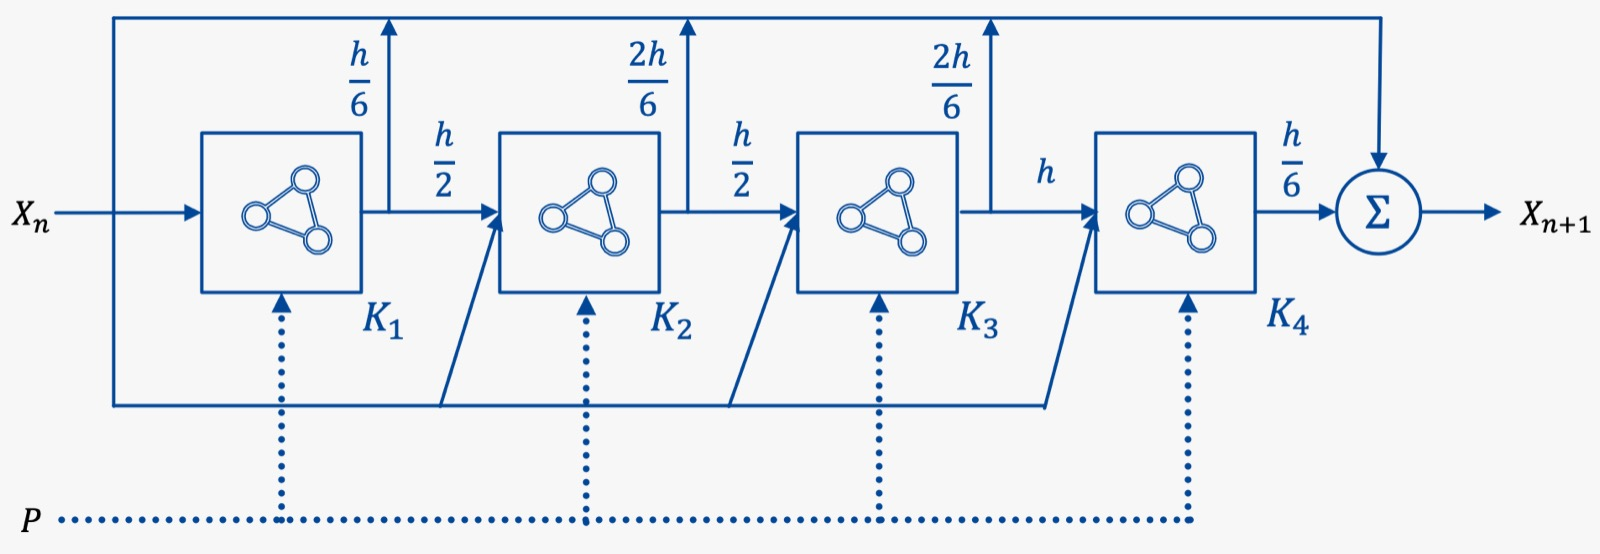
\includegraphics[width=.7\linewidth]{figures/runge_kutta/net_architecture}
	\end{figure}
\end{frame}

\begin{frame}
	\frametitle{Network configuration}
	\centering
	\begin{tabular} { c | c | c | c}
		& Linear System & Andronov-Hopf & R\"ossler attractor	\\
		\hline
		Input			& 2 		& 2			& 3			\\
		\hline
		Parameters		& 0			& 1			& 1			\\
		\hline
		Hidden layers	& 2			& 3			& 3			\\
		\hline
		Neurons / layer	& 20		& 64		& 200		\\
		\hline
		Output			& 2			& 2			& 2			\\
		\hline
		Loss function	& MSE		& MSE		& MSE		\\
		\hline
		Optimization	& SGD		& Adam		& Adam		\\
	\end{tabular}
\end{frame}
